%Romain De Givry

\documentclass[a4paper,12pt]{article}

                %Package imports
\usepackage[utf8]{inputenc}
\usepackage[british]{babel}
\usepackage{multicol}
\usepackage{enumerate}% http://ctan.org/pkg/enumerate
\usepackage{lmodern}
\usepackage{fancyhdr}
\usepackage{lipsum}
\usepackage{titlesec}
%\usepackage{natbib} %Bibliography package to use Harvard referencing
\usepackage{graphicx} % Support for pictures
\usepackage{float}
\usepackage{tabu}
\usepackage{gensymb}
\usepackage{textcomp}
\usepackage{amsmath,amssymb}
\usepackage{caption}
\usepackage{wrapfig} % Wrapping figures
\usepackage{subfig} % Multiple figures
\usepackage[numbib,nottoc]{tocbibind} % Label the reference section
\usepackage{comment} %comment out large sections of text
\usepackage{color} %bring colour
\usepackage{pdflscape} %Change page orientation to landscape
\usepackage{everypage}
\usepackage{url}
\usepackage{hyperref} % links references to destination
\usepackage[intoc]{nomencl} %nomenclature support

%Document geometry 
\usepackage{geometry}
\geometry{a4paper,left=20mm,
right=20mm,
top=20mm,
bottom=20mm,}

%Numbering pages correctly on landscape pages
\newcommand{\Lpagenumber}{\ifdim\textwidth=\linewidth\else\bgroup
  \dimendef\margin=0 %use \margin instead of \dimen0
  \ifodd\value{page}\margin=\oddsidemargin
  \else\margin=\evensidemargin
  \fi
  \raisebox{\dimexpr -\topmargin-\headheight-\headsep-0.5\linewidth}[0pt][0pt]{%
    \rlap{\hspace{\dimexpr \margin+\textheight+\footskip}%
    \llap{\rotatebox{90}{\thepage}}}}%
\egroup\fi}
\AddEverypageHook{\Lpagenumber}
%.............


%font control to computer modern sans serif
\renewcommand*\rmdefault{lmss}
%Document properties
\title{\Huge{Progress Report}}
\author{Usman Ammar }
\date{\today}
%Change section sizes
\titleformat*{\section}{\large\bfseries}
\titleformat*{\subsection}{\normalsize\bfseries}
\titleformat*{\subsubsection}{\small\bfseries}
%Line spacing.....................
\renewcommand{\baselinestretch}{1.25}
%.............................
\makenomenclature

\begin{document}
\maketitle
\vspace{-13mm}
\hrulefill 

\begin{center}
   
    \large\textbf{VORTEX RINGS TO COMBAT HOSTILE DRONES} \\
    Supervisor : Dr Peter Johnson \\
    Associate Supervisor: Dr Andrew Marquis \\
    Word Count:582 \textcolor{red}{TODO: Update this at the end }
\end{center}
 \begin{figure}[h!]
     \centering
     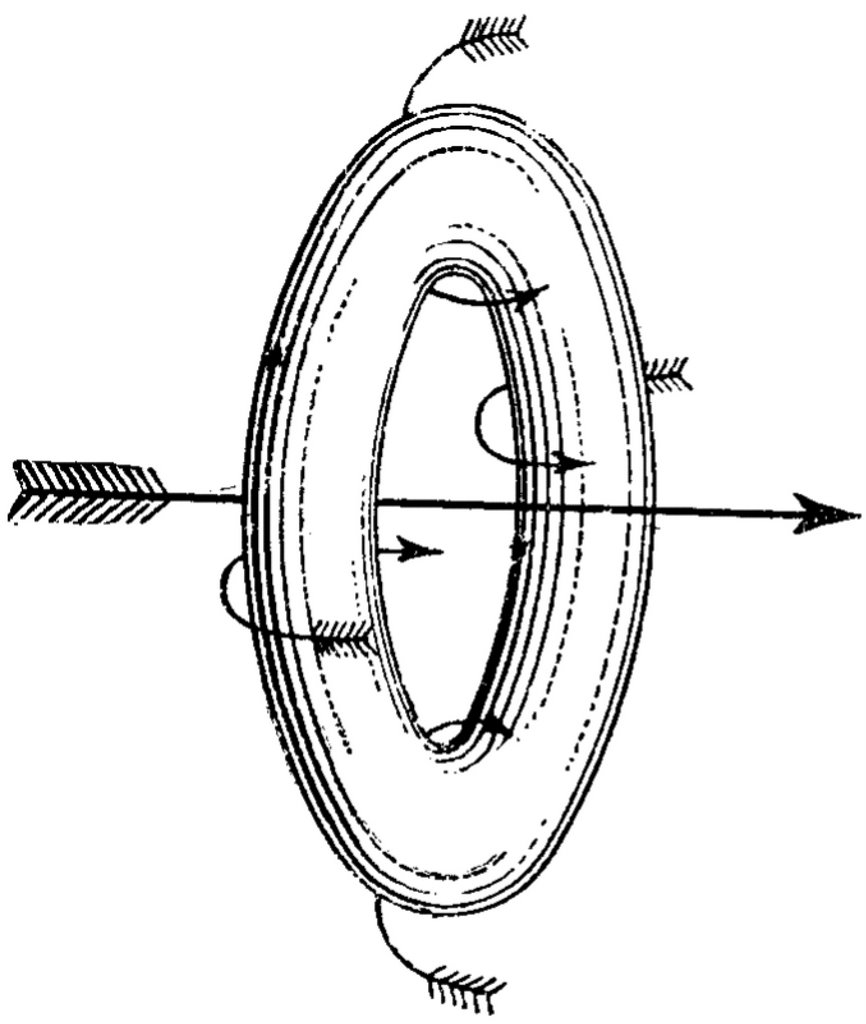
\includegraphics[width=0.7\linewidth]{vortex_titlepage.jpg}
     \caption{\cite{Helmholtz1858}}
     \label{fig:my_label}
 \end{figure}
\newpage
%..................
\section*{Abstract}
\newpage
%....................
\tableofcontents
\newpage
%....................
\nomenclature{$\Gamma$}{Vortex ring circulation}
\nomenclature{$\rho$}{Density}
\nomenclature{$a$}{Core radius}
\nomenclature{$K$}{Kinetic Energy}
\nomenclature{$V$}{Self-induced velocity}
\nomenclature{$P$}{Impulse}
\nomenclature{$E$}{Total Energy}
\nomenclature{$\nu$}{Kinematic Viscosity}
\nomenclature{$T$}{Piston stroke time}
\nomenclature{$\Omega_p$}{Volume of fluid swept out by piston}
\nomenclature{$\Omega_b$}{ Volume of spheroid}
\nomenclature{$\Omega_r$}{Volume of inner-spheroid}
\nomenclature{$M_i$}{Induced mass}
\nomenclature{$\eta$}{Entrainment fluid fraction}
\nomenclature{$C_{dc}$}{Vortex core drag coefficient}
\nomenclature{$D_f$}{Drag force}
\nomenclature{$c$}{Damping coefficient}
\nomenclature{$L$}{Stroke length}
\nomenclature{$D_0$}{Orifice diameter}
\nomenclature{$L/D_0$}{Formation time}
\nomenclature{$u_p$}{instantaneous piston velocity}
\nomenclature{$\Bar{U_p}$}{Running mean of the piston velocity}
\nomenclature{$R_b$}{Semi-major axis}
\nomenclature{$R$}{Ring radius}
\nomenclature{$\gamma$}{Eccentricity}
 \printnomenclature
 \newpage
 %......................
\section{Introduction}
 Drones pose an ever growing threat to the public whether through accident or malicious intents. When the project was initially set up, there had been isolated cases of near misses between drones and planes and a particular case was discussed when a drone disrupted flights at Gatwick in July 2017 for about 14 minutes \cite{RefWorks:42}. Fast forward to today and everyone's heard of the drones that managed to shut down an airport for approximately $36$ hours and causing about a $1,000$ cancellations and coincidentally the airport was again Gatwick \cite{Gatwick}. No one can dispute that drones pose a serious threat to airports most of whom are inadequately prepared for situations like this. In this instance Gatwick had committed to spending £5 million in anti-drone technology.
\vspace{\baselineskip}

\noindent One possible method we're exploring is using vortex rings to shoot down these drones at airports.

\section{Literature Review}
There are few main parameters that characterise vortex rings and these are:
\begin{itemize}
    \item Circulation ($\Gamma$)
    \item Stroke Length (L)
    \item Orifice Diameter (D)
\end{itemize}

The stroke length is a feature of the piston velocity and is calculated through equation \ref{stroke_length}. The running mean of the piston velocity ($\Bar{U_p}$) can be calculated by integrating the taking the average of the instantaneous velocity ($u_p$) over the time period. The Reynolds number for vortex rings is a function of the circulation and kinematic viscosity ($Re = \Gamma / \nu$).

\begin{equation}
    L = \int^t_0 u_p(t)dt
    \label{stroke_length}
\end{equation}

\begin{equation}
    \Bar{U_p} = \left(\frac{1}{t} \int^t_0 u_p dt \right)
    \label{mean_velocity}
\end{equation}

The key parameter to predict what type of vortex ring will form is called the formation time and it is the ratio of the stroke length (L) to the orifice diameter (D).

\begin{equation}
    \frac{L}{D} = \frac{\int^t_0 u_p(t)dt}{D} = \frac{\Bar{U_p} t}{D}
\end{equation}

\begin{figure}[ht]
\centering
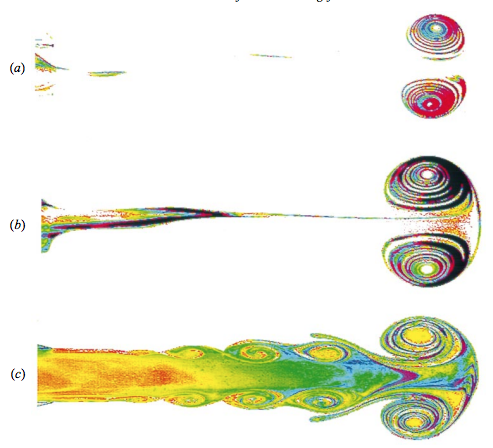
\includegraphics[width=0.8\linewidth]{formation_time.png}
\caption{Vortex Rings at different formation times \cite{universal_timescale}}
\label{fig:formation_time}
\end{figure}

Figure \ref{fig:formation_time} shows vortex rings at three different formation times: 2, 3.8 and 14.5 respectively. Figure \ref{fig:formation_time} is a flow visualisation carried out using Particle Image Velocimetry (PIV) by Gharib, Rambod and Shariff in 1998 \cite{universal_timescale}. In figure \ref{fig:formation_time} (a) we can see that the vortex ring has a negligible (almost zero) trailing jet ; (b) similarly has a small trailing jet while (c) has a massive trailing jet. It can also be observed that the size of the leading vortex in (c) is the same size as (b) despite the larger formation number while the leading vortex in (b) and (c) is bigger than (a). This indicates that beyond a certain formation number vorticity is no longer entrained and is instead shed into the trailing jet. Further tests carried out by Gharib, Rambod and Shariff showed that the maximum circulation the leading vortex can attain is at formation numbers of about 4 and 5 beyond which any extra circulation is shed into the trailing jet. This illustrates that for any potential cannon, increasing the amount of energy given to the flow will not always lead to an increase in circulation of the leading vortex ring and as such this must be accounted for in the design.
\newpage
\section{Deriving Analytical Model}
An analytical model was developed following the methodology by Sullivan, Niemela, Hershberger, Bolster and Donnelly in 2008 in their paper "Dynamics of thin vortex rings" \cite{dynamics_thin_vortexrings}. The model assumes that the core radius (a) is much smaller than the radius of the vortex ring ($a << R$).


\begin{figure}[ht]
\centering
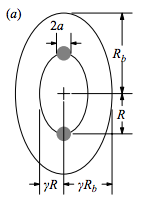
\includegraphics[width=0.3\linewidth]{vortexring_spec.png}
\caption{Vortex Ring Sketch \cite{dynamics_thin_vortexrings}}
\label{fig:vortexring_spec}
\end{figure}

Its assumed the vortex ring is an ellipsoid where $R_b$ and $\gamma R_b$ are the semi-major and semi-minor axes respectively and $\gamma$ is the eccentricity.

\begin{equation}
    K = \frac{1}{2} \rho \Gamma^2 R \bigg[\ln{\frac{8R}{a}} - 2\bigg]
    \label{kinetic_energy}
\end{equation}

\begin{equation}
    V = \frac{\Gamma}{4\pi R} \left( \ln{\frac{8R}{a} - \frac{1}{2}}\right)
    \label{selfinduced_velocity}
\end{equation}


\newpage
\section{Equations}







\vspace{\baselineskip}
\begin{equation}
    E = \frac{1}{2} \rho R \Gamma^{2}\bigg[\ln{\frac{8}{\epsilon}} - \frac{7}{4} + \frac{3}{16} \epsilon^{2} \ln{\frac{8}{\epsilon}} \bigg]
\end{equation}
Where $\Gamma$ is the circulation and $a$ is the core radius.\cite{dynamics_thin_vortexrings}
\textcolor{red}{TODO: reference equation maybe?}
\newpage
\bibliographystyle{unsrt}
\bibliography{export.bib}

\end{document}